% Licensed under the Creative Commons Attribution Share Alike 4.0 International.
% See the LICENSE file in the repository root for full license text.

\section{实验:构建包含多个源文件的程序}

包含多个源文件的 C++ 程序\emph{构建(build)}流程可以图 \ref{fig:build-flow} 示意。该图将构建流程概括为以下三个步骤。

\begin{enumerate}
	\item \emph{预处理(preprocess)}。\emph{预处理器(preprocessor)}处理源文件中的 \lstinline[language={[17]C++}]{#include}、\lstinline[language={[17]C++}]{#define} 等预处理指令,对 \lstinline[language={[17]C++}]{#include} 指令、宏指令进行\textbf{文本替换}。
	\item \emph{编译(compile)}。\emph{编译器(compiler)}\textbf{独立地}处理各源文件,将每个源文件编译为中间文件。
	\item \emph{链接(link)}。\emph{链接器(linker)}处理\textbf{所有}需要的中间文件,最后生成可执行文件。
\end{enumerate}

\begin{figure}
	\centering
	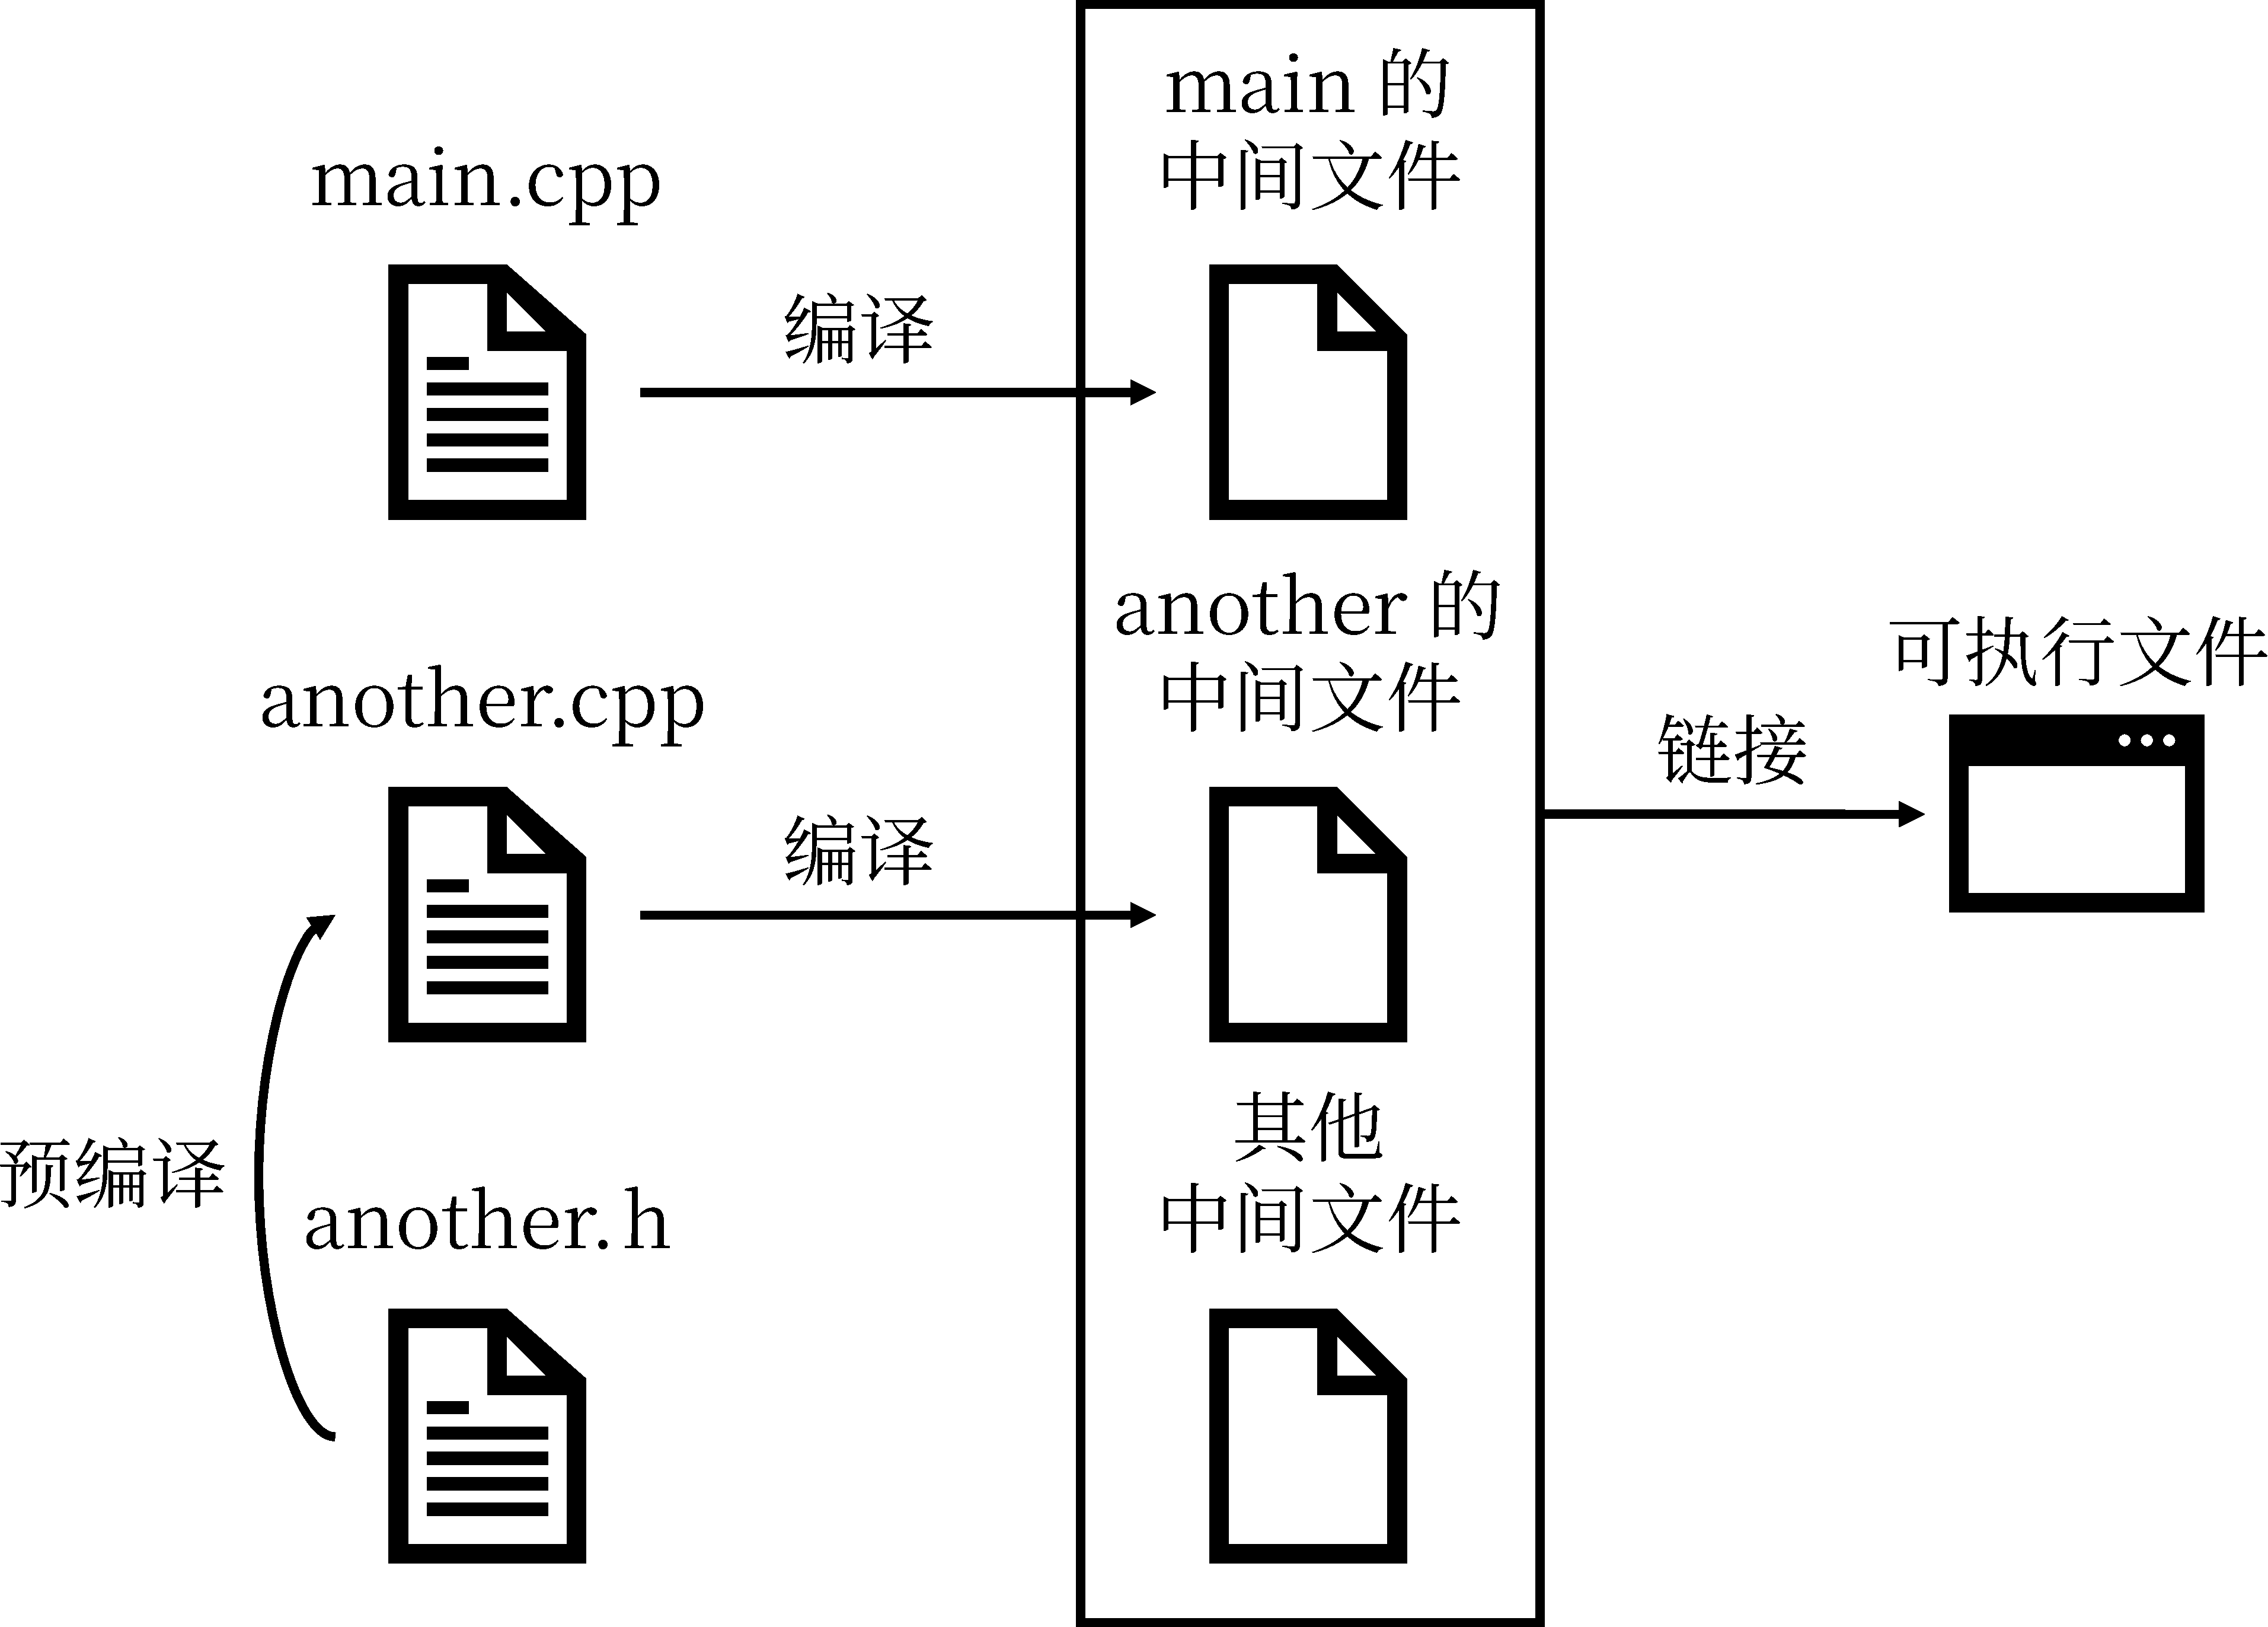
\includegraphics[scale=0.15]{assets/build-flow}
	\caption{多个 C++ 源文件的构建流程示意图。}
	\label{fig:build-flow}
\end{figure}

一般认为,C++ 程序的构建流程\footnote{没有讨论单个源文件经过编译得到单个中间文件时,习惯上用“编译”替代“构建”。}包括预处理、编译、汇编、链接四个步骤,此处我们将汇编这一步骤并入编译,以突出之后的实验要讨论的问题。

\subsection*{实验步骤}

\begin{enumerate}
	\item
\end{enumerate}
